\documentclass[11pt]{article}
% --- Encoding e font ---
\usepackage[utf8]{inputenc}
\usepackage[T1]{fontenc}
\usepackage{lmodern}

% --- Matematica ---
\usepackage{amsmath,amssymb,amsfonts,gensymb,amsthm}
\DeclareMathOperator*{\argmin}{arg\,min}
\DeclareMathOperator*{\argmax}{arg\,max}
\usepackage{centernot}
% --- Grafica, colori, float ---
\usepackage{graphicx}
\usepackage[dvipsnames]{xcolor}
\usepackage{float}
% --- Liste e ambienti ---
\usepackage{enumitem}
% --- Caption, numerazione figure ---
\usepackage{caption}
\usepackage{chngcntr}
% --- Caption, numerazione figure ---
\captionsetup{font=small, labelfont=bf, textfont=it}
% --- Indice/TOC personalizzazione (se ti serve) ---
\usepackage{tocloft}
% --- colorbox
\usepackage[most]{tcolorbox}
%--- spazio tra le riga
\usepackage{parskip}
\setlength{\parskip}{0.15cm}
% Elenchi compatti:
\setlist[itemize]{ topsep=2pt, itemsep=0pt, parsep=0pt}
\setlist[enumerate]{topsep=2pt, itemsep=0pt, parsep=0pt}

% Per il codice
\usepackage{listings}
% Definisci i colori esatti di VS Code (tema Light+)
\definecolor{vscodeblue}{RGB}{0,0,255}          % Keywords
\definecolor{vscodeorange}{RGB}{163,21,21}      % Strings
\definecolor{vscodegreen}{RGB}{0,128,0}         % Comments
\definecolor{vscodepurple}{RGB}{197,134,192}    % Control flow e import
\definecolor{vscodeyellow}{RGB}{121,94,38}      % Functions
\definecolor{vscodebg}{RGB}{255,255,255}        % Background
\definecolor{vscodeframe}{RGB}{200,200,200}     % Frame

% Configurazione Python stile VS Code
\lstdefinestyle{vscode}{
    language=Python,
    alsoletter={.},
    backgroundcolor=\color{vscodebg},
    commentstyle=\color{vscodegreen}\itshape,
    numberstyle=\tiny\color{gray},
    stringstyle=\color{vscodeorange},
    basicstyle=\ttfamily\small,
    breakatwhitespace=false,
    breaklines=true,
    captionpos=b,
    keepspaces=true,
    numbers=left,
    numbersep=8pt,
    showspaces=false,
    showstringspaces=false,
    showtabs=false,
    tabsize=4,
    frame=single,
    rulecolor=\color{vscodeframe},
    framesep=10pt,
    xleftmargin=15pt,
    framexleftmargin=15pt,
    % Resetta tutte le keyword e ridefiniscile
    morekeywords={},
    deletekeywords={for,if,while,else,elif,return,break,continue,try,except,finally,with,as,pass,raise,assert,import,from},
    % Keywords blu
    keywordstyle=\color{vscodeblue}\bfseries,
    morekeywords={def,class,lambda,and,or,not,is,in,del,global,nonlocal,yield,await,async,True,False,None,self},
    % Control flow VIOLA
    keywordstyle=[2]\color{vscodepurple}\bfseries,
    morekeywords=[2]{for,if,while,else,elif,return,break,continue,try,except,finally,with,as,pass,raise,assert,import,from},
    % Funzioni
    emph={sqrt,print,input,range,len,str,int,float,list,dict,set,tuple},
    emphstyle=\color{vscodeyellow}
}
\lstset{style=vscode}

%-- for definition (POI definisci defbox)
\newtcolorbox{defbox}[1]{
    colback=gray!10,
    colframe=gray!50,
    fonttitle=\bfseries,
    coltitle=black,
    title=\mbox{#1},  % Cambiato qui
    sharp corners,
    boxrule=0.5pt, breakable}
%-----
%-----
\usepackage{needspace}
%---- Notebox definition \begin{noteboxtitle}{title}
\newtcolorbox{noteboxtitle}[1]{
    colback=white,
    colframe=black!90,
    boxrule=0.8pt,
    arc=3mm,
    title=#1,
    fonttitle=\bfseries,
    left=5pt,
    right=5pt,
    top=5pt,
    bottom=5pt,
      breakable
}

% --- comment
\usepackage{comment}
% --- Margini ---
\usepackage[a4paper,
    top=2.5cm,
    bottom=2.5cm,
    left=2.5cm,
    right=2.5cm,
    bindingoffset=0.5cm
]{geometry}
% --- Titolo con immagine (opzionale) ---
\usepackage{titlepic} % solo se usi \titlepic
% --- Hyperref VA QUASI SEMPRE PER ULTIMO ---
\usepackage{hyperref}
\usepackage{adjustbox}
\usepackage{xltabular}
\usepackage{booktabs}
\raggedbottom


%---Per spezzare le tabelle
\usepackage{longtable}


% --- New structure for Example
\newtheoremstyle{smallexample}
  {3pt}% Space above
  {3pt}% Space below
  {\small}% Body font - testo dell'esempio piccolo
  {}% Indent amount
  {\small\bfseries}% Theorem head font - "Example 18.1" piccolo e grassetto
  {.}% Punctuation after theorem head
  {.5em}% Space after theorem head
  {}% Theorem head spec
\theoremstyle{smallexample}
\newtheorem{example}{Example}[section]
\usepackage[version=4]{mhchem}
\graphicspath{{Images/}}

 %% --- Definizione prima pagina 


%%___NEW COMMAND
\newcommand{\vs}{\vspace{0.2\baselineskip}}



%%%--- Librerie per grafici

\usepackage{tikz}
\usetikzlibrary{positioning, arrows.meta, shapes.geometric, calc}
\usepackage{tcolorbox}
\tcbuselibrary{breakable, skins}



\parindent 0px
\title{\Huge Data Mining and Machine Learning}
\author{\Large Gennaro Basile}
\date{\today}

\titlepic{
    \begin{center}
        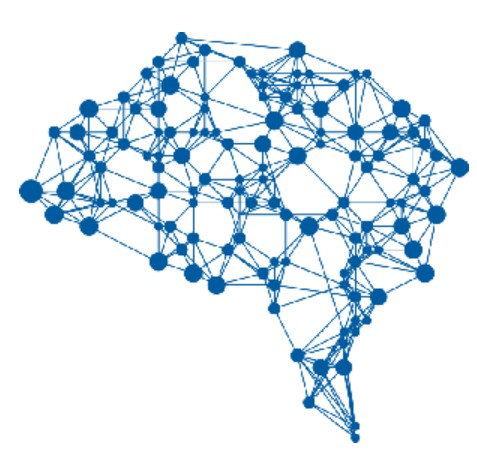
\includegraphics[scale=1]{0.DeepLearningLogo.jpg}
    \end{center}}



\begin{document}
\maketitle
\counterwithin{figure}{subsection}
\captionsetup[figure]{labelfont=bf}

\pagebreak

%% -- Sommario
\tableofcontents
\pagebreak



\section{ML Historical Background}
While modern AI runs on advanced hardware, its theoretical roots stretch back thousands of years. This document highlights the historical milestones that directly shaped the logic, algorithms, and data paradigms used in Data Science today.

\subsection{The Origins: Early Ideas and Ancient Precursors}

\subsubsection{The Birth of Algorithms and Formal Systems}
Long before computers existed, humans developed the conceptual frameworks required for systematic computation and Natural Language Processing (NLP).
\begin{itemize}
    \item \textbf{The Golem (11th-12th Century):} A mythological creature activated by step-by-step instructions. It represents the conceptual forerunner of the \textbf{algorithm}.
    \item \textbf{Panini (6th Century B.C.):} Created a system of rules completely describing the Sanskrit language. This is considered history's first \textbf{formal system} and the theoretical ancestor of modern NLP.
    \item \textbf{Al-Khwarizmi (820 A.D.):} Formalized systematic methods for solving mathematical equations. The word \textbf{algorithm} is a Latinization of his name.
\end{itemize}

\subsubsection{Binary, Zero, and Computational Logic}
Digital computing and logical reasoning rely entirely on binary states and formal mathematical structures.
\begin{itemize}
    \item \textbf{Pingala \& Brahmagupta:} Pingala (c. 300 B.C.) described the first known \textbf{binary} numeral system. Brahmagupta (628 A.D.) introduced \textbf{zero} and negative numbers, making modern computer arithmetic possible.
    \item \textbf{Gottfried Wilhelm Leibniz (17th Century):} Recognized that all computation could be performed using just two states (0 and 1). He also envisioned reducing all human reasoning to a formal symbolic language, anticipating the goals of symbolic AI.
\end{itemize}

\subsubsection{The Nyaya School: Ancient Epistemology meets Modern ML}
Founded in the 2nd Century B.C., this Hindu philosophical system categorized how minds acquire valid knowledge. Its four instruments of knowledge map perfectly to modern AI architecture:
\begin{itemize}
    \item \textbf{Perception :} Direct sensory input. In AI, this maps to \textit{sensor data and input features}.
    \item \textbf{Inference :} Deductive reasoning from premises. This maps to \textit{rule-based logic systems}.
    \item \textbf{Analogy :} Learning by comparing new things to known examples. This maps exactly to the core concept of \textit{Machine Learning and Pattern Recognition}.
    \item \textbf{Testimony:} Knowledge from reliable sources. In data science, this maps to \textit{Data Quality and Data Governance} (your model is only as good as your data source).
\end{itemize}

\subsection{From Mechanical Computation to Formal Logic}
The transition from abstract math to physical computing required machines that could be programmed to change their behavior.
\begin{itemize}
    \item \textbf{Mechanical Automata:} Inventors like Al-Jazari and Pierre Jaquet-Droz built physical machines with variable, programmable behaviors using pegs, gears, and feedback loops.
    \item \textbf{Charles Babbage (19th Century):} Designed the \textbf{Analytical Engine}, the first concept of a general-purpose computer. It featured an arithmetic unit, memory, and used \textbf{punched cards} for input.
\end{itemize}

\subsubsection{Ada Lovelace and the AI Philosophy (1843)}
Ada Lovelace wrote the first published algorithm for Babbage's machine, making her the world's first programmer. More importantly, she formulated \textbf{Lady Lovelace's Objection}: the idea that a machine can only do what it is explicitly programmed to do and cannot originate anything genuinely new.


This sparked the fundamental debate around artificial creativity. Today, it remains a highly relevant philosophical question when evaluating whether Generative AI truly \textit{creates} or merely recombines its training data.




\subsection{The Limits of Perfect Logic}
For centuries, mathematicians dreamed of reducing all reasoning to mechanical calculation. However, in the 1930s, this dream was mathematically proven to be impossible.

\begin{itemize}
    \item \textbf{G\"odel's Incompleteness Theorems (1931):} Proved that in any sufficiently complex logical system, there are statements that are true but \textit{impossible to prove}.
    \item \textbf{Turing's Halting Problem (1936):} Proved that there is no universal algorithm that can solve every computational problem. 
\end{itemize}
\textbf{Data Science Takeaway:} These theorems proved that we cannot build an AI that perfectly deduces the truth for complex, real-world problems using only rigid rules. There is a hard theoretical ceiling to purely logical programming.

\subsubsection{Symbolic vs. Connectionist AI}
The failure of \textit{perfect logic} split AI into two distinct philosophies:

\begin{enumerate}
    \item \textbf{Symbolic AI (Rule-Based):} Assumes intelligence comes from manipulating symbols using formal, hand-coded rules (e.g., \textit{If A, then B}). It struggles with uncertainty and complex, messy real-world data.
    \item \textbf{Connectionist AI (Data-Driven):} Inspired by the brain. It acknowledges that we cannot write perfect rules for everything. Instead, it seeks to \textbf{learn approximate patterns from data}. This is the foundation of modern Machine Learning and Deep Learning.
\end{enumerate}

\subsection{The Pioneers of Connectionism (1943--1956)}
To build a Connectionist AI, scientists needed a new architecture.
\begin{itemize}
    \item \textbf{McCulloch-Pitts Neuron (1943):} The first mathematical model of a brain cell. It took binary inputs, summed them up, and \textit{fired} (output a 1) only if the sum crossed a certain threshold.
    \item \textbf{Hebbian Learning (1949):} Donald Hebb introduced the first learning rule: \textit{"Neurons that fire together, wire together."} He showed that network connections (weights) could be mathematically strengthened based on the correlation between inputs and outputs: 
    $$w_i^{(\text{new})} = w_i^{(\text{old})} + x_i \cdot y$$
    \item \textbf{Dartmouth Conference (1956):} The official founding moment of Artificial Intelligence as an academic field.
\end{itemize}

\subsubsection{The Anatomy of an Artificial Neuron}
By the late 1950s, the artificial neuron was formalized into the exact mathematical operator we still use in Data Science today. It is a two-step process:

Given an input vector $\mathbf{x} = (x_1, \dots, x_M)$ and a weight vector $\mathbf{w} = (w_1, \dots, w_M)$:

\textbf{Step 1: Pre-activation (Linear Combination)}.
The neuron calculates the weighted sum of its inputs (often adding a bias term, though omitted here for simplicity):
\begin{equation}
z = \sum_{i=1}^{M} w_i \, x_i
\end{equation}





\textbf{Step 2: Activation (Non-Linearity)}.
The neuron passes that sum through a non-linear activation function $f$ (like Sigmoid or ReLU) to get the final output:
$$y = f(z)$$





\textbf{Why the Non-Linear function $f$ is crucial:} 
If $f$ were just a linear function (e.g., $f(z) = z$), then stacking 100 layers of neurons would still just result in a basic linear regression model. The non-linear activation function is the secret ingredient that allows neural networks to learn highly complex, curved boundaries in the data.





This extremely simple operator, a non-linear function of a linear combination, is the fundamental building block of all neural networks, from the simplest perceptron of the 1950s to the largest transformer models of today. 

\subsection{The Perceptron}
In 1958, \textbf{Frank Rosenblatt}, a psychologist working at Cornell University, published a preliminary paper introducing a new computational model.
His goal was surprisingly biological: he wanted to model the simple decision system present in the eye of a fly.
He called his invention the \textbf{Perceptron}.



\begin{defbox}{Perceptron (Rosenblatt, 1958)}
A \textbf{perceptron} is the simplest form of artificial neural network.  
It is a single computational unit that:
\begin{enumerate}
    \item receives an input vector $\mathbf{x} = (x_1, x_2, \dots, x_n)$;
    \item multiplies each input by a corresponding weight $w_j$;
    \item computes the weighted sum $\displaystyle\sum_{j} w_j\, x_j$;
    \item compares the result with a threshold $t \in \mathbb{R}$;
    \item produces a binary output: $0$ or $1$.
\end{enumerate}
\end{defbox}

It acts as a binary classifier, taking multiple inputs, weighting them, and passing them through a hard threshold (a step function) to output either a 0 or a 1.


Formally, the output rule is:

\begin{equation}
\text{output} =
\begin{cases}
0 & \text{if } \displaystyle\sum_{j} w_j\, x_j < t \\[6pt]
1 & \text{if } \displaystyle\sum_{j} w_j\, x_j > t
\end{cases}
\end{equation}


         \begin{figure}[H] 
        \centering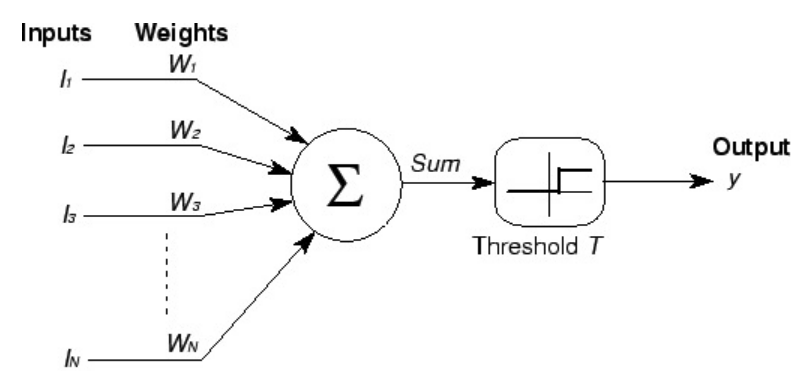
\includegraphics[scale=0.3]{3.Scheme of a perceptron.jpeg}
        \caption{Scheme of a perceptron}
    \captionsetup{font=footnotesize}
    \end{figure}







\subsubsection{Mathematical \& Geometric Formulation}
To make the math elegant and ready for optimization, the threshold is typically moved to the left side of the equation and treated as a \textbf{bias} ($b$). Using vector dot-product notation, the perceptron rule is:

\begin{equation}
\text{Output} =
\begin{cases}
0 & \text{if } \mathbf{w} \cdot \mathbf{x} + b \leq 0 \\
1 & \text{if } \mathbf{w} \cdot \mathbf{x} + b > 0
\end{cases}
\end{equation}



\textbf{Crucial Data Science Concept: The Linear Decision Boundary}\\
Geometrically, the equation $\mathbf{w} \cdot \mathbf{x} + b = 0$ defines a \textbf{hyperplane} (a line in 2D, a plane in 3D). The perceptron puts all "1" predictions on one side of this line, and all "0" predictions on the other. Therefore, a single perceptron can \textit{only} solve \textbf{linearly separable} problems.

\vs

\begin{example}{\textbf{buy a car}}

Imagine you want to buy a car and your decision depends on three factors, ranked by importance:

\begin{enumerate}
    \item \textbf{Number of passengers} (most important): you have three kids, so you need at least 5 seats.  
    Set $x_3 = 1$ if the car has $\geq 5$ seats, $0$ otherwise.
    \item \textbf{Cost}: you want to spend as little as possible.  
    Set $x_1 = 1$ if the price is below 25\,000\ euro $0$ otherwise.
    \item \textbf{Performance}: you want sporty driving.  
    Set $x_2 = 1$ if the car is sporty, $0$ otherwise.
\end{enumerate}

Weights reflecting the ranking: $w_3 = 4,\; w_1 = 2,\; w_2 = 1$.  
Threshold: $t = 5$.

Now the perceptron computes $w_1 x_1 + w_2 x_2 + w_3 x_3$ and checks whether the sum exceeds~5.
For example, a cheap sporty 5-seater gives $2(1)+1(1)+4(1)=7>5 \Rightarrow$ output $=1$ (buy!).
A cheap sporty 4-seater gives $2(1)+1(1)+4(0)=3<5 \Rightarrow$ output $=0$ (don't buy).

This is the simplest way to automate a decision-making process, but simple solutions very seldom work in real life.
\end{example}



\subsection{The First Neural Winter \& The XOR Problem}
In the late 1960s, AI research funding dried up, leading to the \textit{First Neural Winter.} While overpromising and hardware limitations played a role, the technical fatal blow came from Minsky and Papert in 1969, who proved the limitations of the single-layer perceptron.

\subsection{The XOR Problem: The Limit of Linear Inseparability}
To truly understand why the First Neural Winter happened, we must look closely at the XOR (Exclusive OR) problem. It mathematically proved that a single-layer perceptron is fundamentally limited.


Consider two binary inputs, $x_1$ and $x_2$. The XOR logic gate outputs a $1$ \textit{only} if the inputs are strictly different from each other:
\begin{center}
\begin{tabular}{|c|c|c|}
\hline
$x_1$ & $x_2$ & \textbf{XOR Output} \\
\hline
0 & 0 & \textbf{0} \\
1 & 0 & \textbf{1} \\
0 & 1 & \textbf{1} \\
1 & 1 & \textbf{0} \\
\hline
\end{tabular}
\end{center}

\vs

\textbf{The Geometric Proof}\\
Imagine plotting these four input pairs on a 2D Cartesian graph, where $x_1$ is the horizontal axis and $x_2$ is the vertical axis.
\begin{itemize}
    \item The points $(0,0)$ and $(1,1)$ belong to \textbf{Class 0}.
    \item The points $(1,0)$ and $(0,1)$ belong to \textbf{Class 1}.
\end{itemize}
If you visualize this, Class 1 points lie on one diagonal, and Class 0 points lie on the opposite intersecting diagonal. 

\vs
\textbf{The Perceptron's Failure}\\
As established, the mathematical formula of a single perceptron calculates $\mathbf{w} \cdot \mathbf{x} + b = 0$. In geometry, this equation represents a \textbf{single straight line}. The perceptron's only job is to adjust its weights to draw a line that puts all Class 1 points on one side, and all Class 0 points on the other. 

No matter how you rotate, tilt, or shift a single straight line on that graph, \textbf{it is geometrically impossible} to separate the two 1s from the two 0s. Because the data is not \textit{linearly separable}, the single perceptron utterly fails. 

         \begin{figure}[H] 
        \centering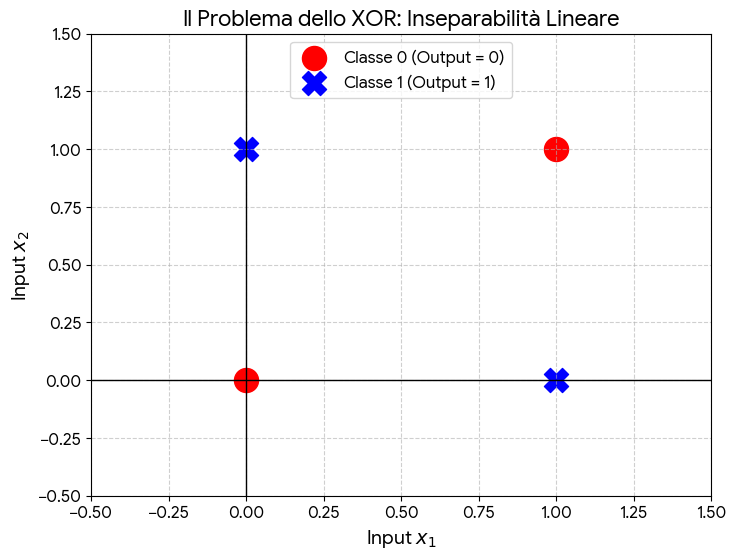
\includegraphics[scale=0.25]{4.Perceptron problem.jpeg}
        \caption{XOR Problem}
    \captionsetup{font=footnotesize}
    \end{figure}

\textbf{Data Science Takeaway:}\\
To solve the XOR problem, you need to draw \textit{multiple} intersecting lines (or non-linear boundaries) to fence off the points. This is exactly why \textbf{Multi-Layer Perceptrons (MLPs)} with hidden layers were invented: each neuron in a hidden layer draws its own line, and the network combines them to solve complex, non-linear problems.


\subsubsection{The Differentiability Crisis}
A deeper technical issue caused the stagnation: \textbf{binary neurons}.
The step function used in early perceptrons jumps instantly from 0 to 1. In calculus, a hard jump is \textbf{not differentiable} (its gradient is either zero or undefined). 

\textit{Why this matters:} If you cannot calculate a gradient, you cannot use optimization algorithms like Gradient Descent to update the weights. To build deeper networks that could solve XOR, researchers eventually realized they had to replace the binary step function with smooth, continuous activation functions.

\subsubsection{Sparks in the Winter: Early Deep Learning}
Despite the winter, a few pioneers laid the groundwork for modern Deep Learning:
\begin{itemize}
    \item \textbf{Ivakhnenko \& Lapa (1965):} Created the first multi-layer perceptron (MLP). They introduced the use of a \textbf{validation set} and \textbf{network pruning}, practices that are mandatory in modern data science.
    \item \textbf{Shun'ichi Amari (1967):} Trained a 5-layer network using \textbf{Stochastic Gradient Descent (SGD)}.
    \item \textbf{Kohonen \& Anderson (1972):} Formulated neural networks using \textbf{matrix mathematics}, establishing the linear algebra foundation that allows modern GPUs to train massive models today.
\end{itemize}

\subsection{The End of the First Winter}
The year 1982 is often considered a major turning point in the history of Artificial Neural Networks (ANNs). After a difficult period, often called the \textbf{First ANN Winter}, several important ideas and models appeared or became popular again. In this period, researchers introduced new neural architectures, improved learning methods, and rebuilt interest in neural computation.


\subsubsection{Self-Organizing Maps (SOMs) - Kohonen, 1982}

In 1982, \textbf{Teuvo Kohonen} introduced the \textbf{Self-Organizing Map (SOM)}. This model is important because it learns to represent high-dimensional data in a lower-dimensional space, usually a two-dimensional grid.

\begin{defbox}{Self-Organizing Map (SOM)}
A \textbf{Self-Organizing Map} is a neural network that transforms high-dimensional input data into a low-dimensional representation while preserving the topological relationships of the data.
\end{defbox}

This means that if two input points are similar in the original space, they should also be close to each other on the map.

SOMs are trained using \textbf{competitive learning}. In competitive learning, neurons compete with each other to respond to an input. The neuron whose weights are closest to the input is called the \textbf{winning neuron}, and it is updated together with its neighbors.

\begin{defbox}{Competitive Learning}
\textbf{Competitive learning} is a training strategy in which neurons compete to become the best match for an input pattern. Only the winning neuron, and usually its neighboring neurons, are updated.
\end{defbox}

The idea of SOMs was inspired by the \textbf{cortical homunculus}, which is a distorted map of the human body in the brain. In the brain, different areas are dedicated to processing sensory information from different body parts, and these areas preserve a type of spatial organization.



\paragraph{Why SOMs are useful}
SOMs are useful because they:
\begin{itemize}
    \item reduce dimensionality,
    \item help visualize complex data,
    \item preserve neighborhood relations,
    \item can discover clusters or patterns in data.
\end{itemize}

         \begin{figure}[H] 
        \centering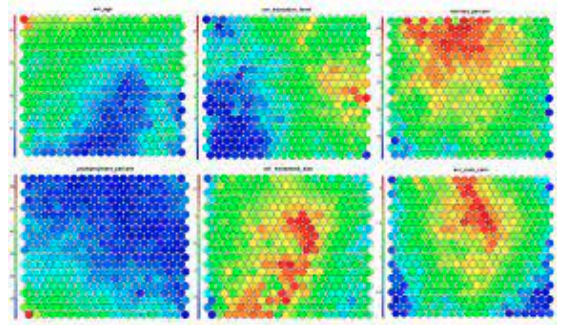
\includegraphics[scale=0.3]{5.Self organizing maps (SOMs).jpeg}
        \caption{Self organizing maps (SOMs)}
    \captionsetup{font=footnotesize}
    \end{figure}

\subsubsection{Recurrent Neural Networks (RNNs) - Hopfield, 1982}1982 can be considered the end of the First ANN Winter. In that year, important problems started to find new solutions.

One of the most important contributions came from \textbf{John Hopfield}, who published the paper \textit{Neural networks and physical systems with emergent collective computational abilities} in 1982.

This work introduced the \textbf{Hopfield Network} as a new important neural model.

\begin{defbox}{Hopfield Network}
A \textbf{Hopfield Network} is a recurrent neural network with feedback connections, designed as an associative memory system. It can store patterns and retrieve them from partial or noisy inputs.
\end{defbox}

A Hopfield Network is recurrent because connections form loops. The output of neurons can influence the network again, unlike in a simple feedforward network where information moves only from input to output.

\begin{defbox}{Recurrent Neural Network (RNN)}
A \textbf{Recurrent Neural Network} is a neural network in which connections form cycles, allowing the network to keep information from previous steps and process sequential or dynamic data.
\end{defbox}


\paragraph{Main idea}
The important message is that recurrent networks can model systems with memory. This is essential for tasks where the order of information matters, such as time series, language, or pattern completion.

\subsubsection{Hybrid Networks and the US--Japan Conference}

In the same year, 1982, \textbf{Reilly and Cooper} introduced a \textbf{hybrid network}.

\begin{defbox}{Hybrid Network}
A \textbf{hybrid network} is a neural architecture composed of multiple layers or components, where different parts of the system use different problem-solving strategies.
\end{defbox}

The central idea is simple: instead of using the same mechanism everywhere, different layers can do different jobs. This is an important idea because many later AI systems also combine multiple strategies, models, or learning mechanisms.



\subsection{Backpropagation: General Idea}

Backpropagation is one of the most important algorithms in the history of machine learning.

\begin{defbox}{Backpropagation}
\textbf{Backpropagation} is a method used to compute how the weights of a neural network should be updated in order to reduce the prediction error.
\end{defbox}

In simple words, a neural network makes a prediction, compares it with the correct answer, computes the error, and then propagates that error backward through the layers to understand how each weight contributed to the mistake.

This allows the network to improve step by step.

\paragraph{Basic intuition}
The process can be summarized as follows:
\begin{enumerate}
    \item Send the input forward through the network.
    \item Compute the output.
    \item Measure the error between predicted output and true output.
    \item Send the error backward through the network.
    \item Compute how much each weight contributed to the error.
    \item Update the weights.
\end{enumerate}


\subsubsection{Multilayer Perceptron (MLP)}

This chapter focuses on the researchers who made backpropagation practical and standard.

First, \textbf{Paul Werbos} applied backpropagation to \textbf{Multilayer Perceptrons (MLPs)} in the form that later became standard.

\begin{defbox}{Multilayer Perceptron (MLP)}
A \textbf{Multilayer Perceptron} is a feedforward neural network composed of an input layer, one or more hidden layers, and an output layer.
\end{defbox}

Werbos discussed the importance of backpropagation for learning in his PhD work. This was crucial because MLPs need a method to train weights in hidden layers, and simpler learning rules were not enough.

Later, in 1985, \textbf{David Rumelhart}, \textbf{Geoffrey Hinton}, and \textbf{Ronald Williams} published a seminal paper that made backpropagation much more widely known.

\begin{defbox}{Standard Backpropagation}
\textbf{Standard backpropagation} is the learning procedure used in multilayer neural networks where the prediction error is propagated backward through the hidden layers using the chain rule, and the weights are updated by gradient descent.
\end{defbox}

This was a major breakthrough because it solved one of the central limitations of earlier neural networks: how to train hidden layers.

\paragraph{Why was this so important?}
Before backpropagation became popular, single-layer perceptrons were limited. They could not solve many interesting nonlinear problems. Backpropagation made multilayer networks trainable, which opened the door to much more powerful models.


\subsubsection{The Mathematics of Backpropagation}

Backpropagation is simply the application of the \textbf{Chain Rule} from calculus to a neural network. It calculates exactly how much each individual weight contributed to the network's final error.


Suppose we have a loss function \(L\), and we want to update a weight \(w\). Gradient descent uses:
\begin{equation}
w \leftarrow w - \eta \frac{\partial L}{\partial w}
\end{equation}
where:
\begin{itemize}
    \item \(w\) is the weight,
    \item \(\eta\) is the learning rate,
    \item \(\frac{\partial L}{\partial w}\) is the derivative of the loss with respect to the weight.
\end{itemize}

The difficult part is computing \(\frac{\partial L}{\partial w}\) for weights in hidden layers. Backpropagation does exactly this by applying the chain rule layer by layer from the output back to the input.

For example, if
\[
L = L(a^{(2)}), \qquad a^{(2)} = f(z^{(2)}), \qquad z^{(2)} = w a^{(1)} + b
\]
then
\begin{equation}
\frac{\partial L}{\partial w}
=
\frac{\partial L}{\partial a^{(2)}}
\cdot
\frac{\partial a^{(2)}}{\partial z^{(2)}}
\cdot
\frac{\partial z^{(2)}}{\partial w}
\end{equation}



\begin{enumerate}
    \item \textbf{Forward Pass:} The data moves through the network to make a prediction.
    \item \textbf{Calculate Loss:} Compare the prediction to the true target using a Loss Function ($L$).
    \item \textbf{Backward Pass:} Use the chain rule to calculate the gradient of the loss with respect to a specific weight $w$ in a hidden layer:
    $$ \frac{\partial L}{\partial w} = \frac{\partial L}{\partial a} \cdot \frac{\partial a}{\partial z} \cdot \frac{\partial z}{\partial w} $$
    \item \textbf{Gradient Descent:} Update the weight by stepping in the opposite direction of the gradient, scaled by a learning rate ($\eta$):
    $$ w \leftarrow w - \eta \frac{\partial L}{\partial w} $$
\end{enumerate}

\begin{defbox}{The Basic Calculus: The Chain Rule}

In calculus, the \textbf{Chain Rule} is used to calculate the derivative of \textit{composite functions} (functions nested inside other functions).  Suppose a variable $x$ influences $u$, which in turn influences $y$. Mathematically, this is written as:
\begin{equation*}
y = f(u) \quad \text{and} \quad u = g(x) \implies y = f(g(x))
\end{equation*}
If we want to know how a tiny change in $x$ affects the final output $y$, we cannot calculate it directly. Instead, we multiply the derivatives of each individual step:
\begin{equation*}
\frac{dy}{dx} = \frac{dy}{du} \cdot \frac{du}{dx}
\end{equation*}
\textit{Intuition:} If $y$ changes 2 times as fast as $u$, and $u$ changes 3 times as fast as $x$, then $y$ changes $2 \times 3 = 6$ times as fast as $x$.

\paragraph*{The Neural Network Pipeline.}
A single weight in a neural network is just a variable at the very beginning of a nested function. The data flows through three distinct mathematical steps:
\begin{enumerate}
    \item \textbf{Linear Combination ($z$):} The input $x$ is multiplied by the weight $w$ (ignoring the bias for simplicity).
    \begin{equation*}
        z = w \cdot x
    \end{equation*}
    \item \textbf{Activation ($a$):} The result $z$ is passed through a non-linear activation function $f$ (like Sigmoid or ReLU).
    \begin{equation*}
        a = f(z)
    \end{equation*}
    \item \textbf{Loss Function ($L$):} The network's prediction $a$ is compared to the true target $y_{\text{true}}$ to calculate the error.
    \begin{equation*}
        L = \text{Loss}(a, y_{\text{true}})
    \end{equation*}
\end{enumerate}
This creates the chain: $w \rightarrow z \rightarrow a \rightarrow L$.

\paragraph*{Calculating the Gradient via Backpropagation}.
To update our weight $w$ using Gradient Descent, we need to find $\frac{\partial L}{\partial w}$ (the partial derivative of the Loss with respect to the weight). This tells us exactly how much of the final error is \textit{blamed} on this specific weight. By applying the Chain Rule backwards from the output to the input, we get the fundamental equation of Backpropagation:
\begin{equation*}
\frac{\partial L}{\partial w} = \frac{\partial L}{\partial a} \cdot \frac{\partial a}{\partial z} \cdot \frac{\partial z}{\partial w}
\end{equation*}

Let's break down what these three terms actually represent:
\begin{itemize}
    \item $\frac{\partial L}{\partial a}$: \textbf{The Error Derivative.} How much the loss changes if the final prediction changes.
    \item $\frac{\partial a}{\partial z}$: \textbf{The Activation Derivative.} The slope of the activation function at point $z$.
    \item $\frac{\partial z}{\partial w}$: \textbf{The Input Derivative.} Since $z = wx$, the derivative of $z$ with respect to $w$ is simply the original input $x$.
\end{itemize}
Therefore, the gradient of the weight is simply the product of the error, the slope of the activation, and the input value.

\paragraph*{The Mathematical Cause of the Neural Winter}.
Looking at the Backpropagation formula perfectly explains why the First Neural Winter happened. 

Early Perceptrons used a \textbf{binary step function} for their activation $a = f(z)$. A step function is a flat horizontal line that instantly jumps from 0 to 1. In calculus, the derivative (slope) of a flat line is exactly $0$.  If $\frac{\partial a}{\partial z} = 0$, then the entire multiplication chain collapses:
\begin{equation*}
\frac{\partial L}{\partial w} = \frac{\partial L}{\partial a} \cdot 0 \cdot x = 0
\end{equation*}
With a gradient of 0, the network receives no feedback, weights cannot be updated, and the algorithm completely fails to learn. This mathematical roadblock was only solved by replacing step functions with \textit{smooth, differentiable} activation functions (like the Sigmoid curve).


\end{defbox}




\subsubsection{The Second AI Winter (1987--1993)}
While neural networks were advancing theoretically, the corporate world became obsessed with \textbf{Expert Systems}: AI based entirely on rigid, human-coded logical rules (Symbolic AI). 

 General-purpose personal computers became cheaper and more powerful, so expensive dedicated AI machines were less attractive. causing the \textbf{Second AI Winter}. As a result, interest in AI faded again.


        \paragraph*{The Ultimate Historical Takeaway:}
        By the end of the 1980s, the core math and architectures of Deep Learning (MLP, RNN, CNN, SOM, Backpropagation) were completely established. The explosive AI boom we see today is not due to a fundamental change in the math; it is due to massive increases in \textbf{Data Availability} (the Internet) and \textbf{Computational Power} (GPUs).


\subsection{The Advent of Modern Deep Learning (2012--2017)}
The current AI boom was triggered by three massive milestones that proved Deep Learning was superior to older, rule-based methods:

\begin{enumerate}
    \item \textbf{AlexNet (2012):} A deep neural network that shattered records in image recognition. It proved that training large networks on \textbf{GPUs} with massive datasets could solve complex real-world problems.
    \item \textbf{AlphaGo (2016):} Defeated the world champion in Go. This proved neural networks could handle long-term strategic planning and intuition, not just pattern recognition.
    \item \textbf{The Transformer (2017):} A revolutionary architecture invented by Google. Instead of processing data sequentially (word by word), it uses an \textbf{Attention Mechanism} to look at an entire sequence at once. This is the underlying architecture of all modern Large Language Models (LLMs).
\end{enumerate}

\subsubsection{The Generative Era (2022--2023)}
Driven by the maturity of the Transformer architecture, AI shifted from merely \textit{analyzing} data to \textit{creating} new content (text, code, images, audio). 

The release of \textbf{ChatGPT (Nov 2022)} brought LLMs to the public. Shortly after, models became \textbf{Multimodal}, meaning they could process and generate across different data types (vision, sound, text) simultaneously, mirroring human perception.

\subsubsection{The Agentic Turn (2024--Present)}
We are currently transitioning from passive \textit{Generative AI} to proactive \textit{Agentic AI}. 

\begin{itemize}
    \item \textbf{Chatbot (Generative):} Passive. It waits for a prompt, predicts the most likely text response, and resets its memory.
    \item \textbf{Agent (Agentic):} Active and goal-oriented. It possesses \textbf{Persistent Memory}, can perform multi-step reasoning (like the o1 or Gemini 1.5 Pro models), and can autonomously use external tools (like APIs, browsers, or calendars) to execute complete workflows.
\end{itemize}

\subsection{The Model Context Protocol (MCP)}
As Agents become digital workers, they need to communicate with software. \textbf{MCP} is a new standard interface that allows AI agents to securely connect to external tools and databases through one unified layer, rather than requiring custom API integrations for every single app.

\pagebreak
\subsection{Moravec's Paradox and the Common Sense Problem}
To understand the limits of AI, we must look at a historical philosophical problem. 

In 1997, IBM's Deep Blue beat the world chess champion. Chess is mathematically complex, but its rules are perfectly rigid and formal. It is computationally hard, but conceptually easy for a machine. 

Conversely, humans use \textbf{Common-Sense Knowledge}: intuitive, contextual, and unwritten rules about how the physical world works. For decades, Symbolic AI researchers (like the \textbf{CYC Project}) tried to manually type out every single rule of common sense into a database. It failed entirely because the real world is too ambiguous to be hard-coded. 

\textbf{Data Science Takeaway:} This is exactly why we use Deep Learning today. We cannot manually program a car to recognize every possible combination of shadows on a stop sign. We \textit{must} use neural networks to let the machine learn the informal patterns itself.

\subsubsection{Why Automata Still Matter}
If modern AI is all about neural networks learning from data, why do we still study ancient automata and formal rules?
\begin{enumerate}
    \item They prove that intelligence and decision-making can be modeled as \textbf{computation}.
    \item They introduce the foundational concept of \textbf{State and Memory}:crucial for modern recurrent networks and Agents.
    \item They define the absolute \textbf{mathematical limits} of what a machine can and cannot compute (e.g., Turing's Halting Problem).
\end{enumerate}



\pagebreak



  \end{document}